\documentclass{article}
\usepackage{graphicx}
\usepackage{standalone}
\usepackage{multicol}



\begin{document}
    \section{Experimental Results}
     For all of my testing and the results presented I used a 10-dimensional SPHERE function (i.e. $n=10$) with the search space restricted to $[-100,100]^{10}$.

	\subsection{Non-Uniform Mutation with parameter $b \in \{0.05, 1.0, 10.0, 20.0 \} $}
	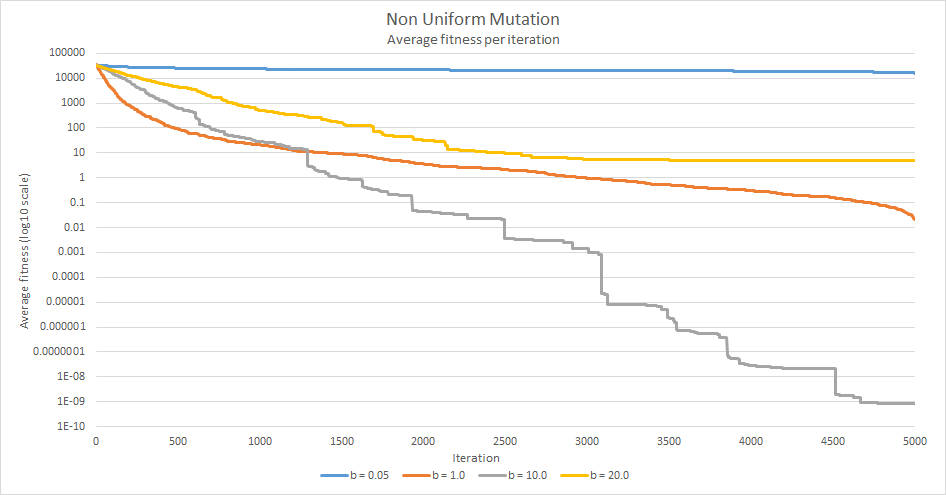
\includegraphics[width=1\textwidth]{Images/NonUniformMutation}\\
	
	As we can see from the graph, for a 10-dimensional sphere function over 5000 iterations the Non-Uniform mutation algorithm did not succeed in finding an optimal solution. The best fitness would have been $0$ but the algorithm does not manage to reach that.\\
	
	The different parameters for $b$ did yield separate and very different results (as shown in the graph). A value of $b=0.05$ produces a very shallow curve with very little reduction in the average fitness value over the 5000 iterations. This proved to be the worst out of all of the parameter values that I tried. This could be due to the way in which the $\Delta(t, y)$ works as the whole second half of the equations is to the exponent $b$. In this case $b=0.05$ which causes the whole equation to become very small, which is then multiplied to the value $y$. This causes a very small overall change in the values of $X$ which could mean that it does not have sufficient time (in the 5000) iterations to deviate very much from its original values.\\
	
	A value of $b=1.0$ produces a rapid initial change (over the first few hundred iterations) which then steadily continues along a constant gradient. The change in the average fitness is greater than with $b=0.05$ and it does get closer to the best average fitness value (with the lowest reached being $0.02$. I believe this is again due to the $\Delta(t, y)$ function as the exponent in this case is $1$ so it is effectively irrelevant. This means that the mutation is directly dependent upon the random number generated for $r$ and the iteration out of the total iterations. This is why it starts to level off after a while, because as $t$ approaches $T$ the value of $r$ approaches $1$ so $\Delta(t, y)$ starts to approach $y \times 1$. This has the effect of not introducing as much variation into each iteration as it would have done at the start of the run.\\
	
	A value of $b=10.0$ produces a constantly declining line which has large jumps in some sections followed by a mini plateau for a while. This value turns out to be the best in my testing as it produced the lowest fitness values out of all of the runs (though it did not achieve the optimal solution). I believe this to be happening because in the $\Delta(t, y)$ equation, $b$ is the exponent, so with this being 10 it is possible to jump large distances between values for $x_i$. However it is not too large so that the value it produces for $x_i$ is either above or below the range $[-100, 100]$ and so would be truncated at the maximum/minimum values. This allows it to gradually step down from its local value.\\
	
	A value of $b=20.0$ produced a very high line on the graph. Is is a worse solution than both $b=1.0$ \& $b=10.0$ however it is better than $b=0.05$. I believe this is due to the $\Delta(t, y)$ equation, $b$ is the exponent, so with this being 20 it is possible to jump large distances between values for $x_i$. In the majority of cases this might push it over the threshold range $[-100, 100]$ which would cause it to be set to the maximum/minimum value. As there is a 50\% chance that either of these cases can happen, and as the value is hitting max/min thresholds often the line tends to stagnate and not vary as much as it could do. This causes it to not seek as many solutions and limits its reach for the best fitness value.\\
	
	From all of this testing I believe that their is a trend that can be seen from the data. \\
	\begin{center}
	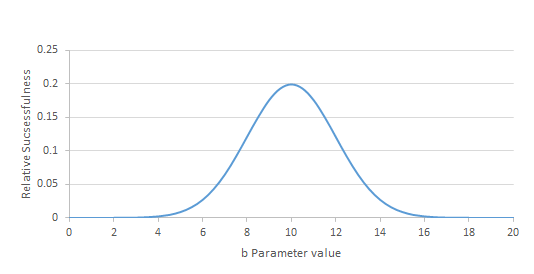
\includegraphics[width=0.8\textwidth]{Images/NonUniformMutationBellCurve}
	\end{center}
	This graph shows the relative successfulness of the algorithm against its $b$ parameter. I would expect that a $b$ value around $10$ to produce the best results and as you go either side of this you start to produce a worse solution.
	
	\subsection{Gaussian mutation without 1/5-rule and parameter $\sigma \in \{0.05, 0.5, 1.0, 10.0\}$}
	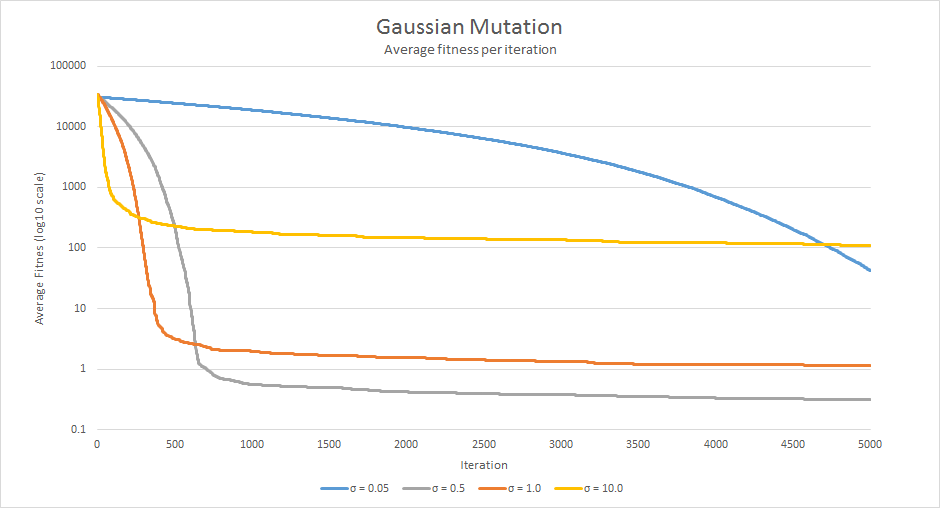
\includegraphics[width=1\textwidth]{Images/GaussianMutation}\\
	
    As we can see from the graph, for a 10-dimensional sphere function over 5000 iterations the Gaussian mutation algorithm did not succeed in finding an optimal solution. The best fitness would have been $0$ but the algorithm does not manage to reach that.\\
	
	The different parameters for $\sigma$ did yield separate and very different results (as shown in the graph). A value of $\sigma=0.05$ produces a very shallow curve (comparably) with a gradual reduction in the average fitness as the iterations continue. This is likely to be because $\sigma$ is very small so the equation $x_i = x_i + \sigma \times m_i$ will have a very small quantity added to it, so it will not vary very much.\\
	
	A value of $\sigma=0.5$ produces better results, a very steep drop over the first few hundred iterations followed by a plateau of very little change. This produced the best result as it achieved the lowest average fitness value.\\
	
	A value of $\sigma=1.0$ produces similar results to $\sigma=0.5$, a very steep drop over the first few hundred iterations followed by a plateau of very little change. However it did not find a fitness value quite as low and was about $3\times$ worse.\\
	
	Finally, a value of $\sigma=10.0$ produces a very steep initial search over just a couple of hundred iterations. However it soon levels out and then there is not much change for the remainder of the 5000 iterations.
	
	\subsection{Comparison of Uniform Mutation, Gaussian mutation with 1/5 rule and the ‘best’ parameter setting for non-uniform and Gaussian mutation without 1/5 rule.}
	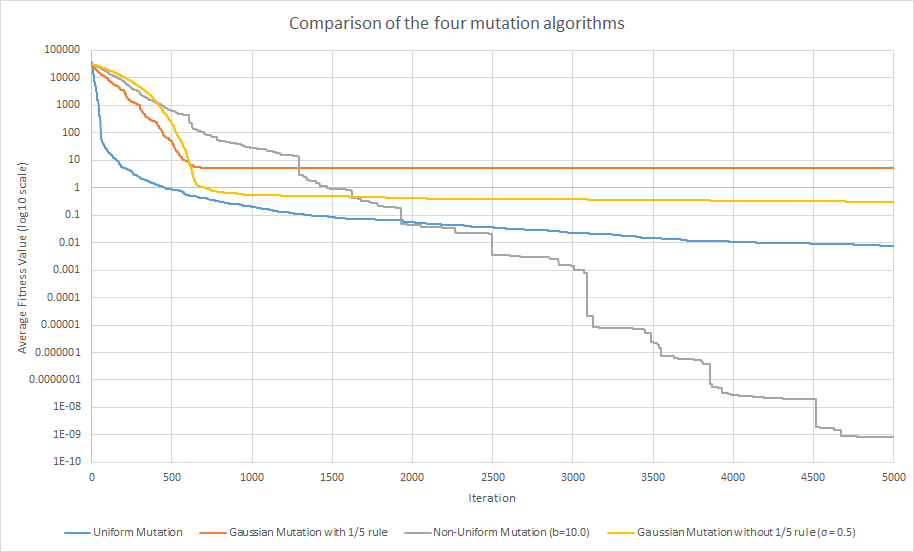
\includegraphics[width=1\textwidth]{Images/ComparisonOfAlgorithms}\\
	
	This comparison graph of all of the four different mutation algorithms (choosing the best parameters in the case of Non-Uniform and Gaussian mutation without 1/5 rule) shows clearly that one of the algorithms far surpasses the others in terms of finding the best fitness value. That is the Non-Uniform mutation algorithms with a parameter of $b=10.0$.\\
	
	We can also see how the others compare to each other, with Uniform Mutation coming in 2\textsuperscript{nd} (though far behind 1\textsuperscript{st} place). 3\textsuperscript{rd} going to Gaussian Mutation without 1/5 rule and a parameter of $\sigma=0.5$. And finally Gaussian Mutation with 1/5 rule coming in last.
	
	
	
\end{document}